\documentclass{article}


% if you need to pass options to natbib, use, e.g.:
%     \PassOptionsToPackage{numbers, compress}{natbib}
% before loading neurips_2022


% ready for submission
% \usepackage{neurips_2022}


% to compile a preprint version, e.g., for submission to arXiv, add add the
% [preprint] option:
\usepackage[preprint]{neurips_2022}


% to compile a camera-ready version, add the [final] option, e.g.:
%     \usepackage[final]{neurips_2022}


% to avoid loading the natbib package, add option nonatbib:
%    \usepackage[nonatbib]{neurips_2022}


\usepackage[utf8]{inputenc} % allow utf-8 input
\usepackage[T1]{fontenc}    % use 8-bit T1 fonts
\usepackage{hyperref}       % hyperlinks
\usepackage{url}            % simple URL typesetting
\usepackage{booktabs}       % professional-quality tables
\usepackage{amsfonts}       % blackboard math symbols
\usepackage{nicefrac}       % compact symbols for 1/2, etc.
\usepackage{microtype}      % microtypography
\usepackage{xcolor}         % colors
\usepackage{makecell}
\usepackage{graphicx}
\graphicspath{{figures}}
\title{Formatting Instructions For NeurIPS 2022}


% The \author macro works with any number of authors. There are two commands
% used to separate the names and addresses of multiple authors: \And and \AND.
%
% Using \And between authors leaves it to LaTeX to determine where to break the
% lines. Using \AND forces a line break at that point. So, if LaTeX puts 3 of 4
% authors names on the first line, and the last on the second line, try using
% \AND instead of \And before the third author name.


\author{%
  Tianyu Xie \\
  School of Mathematical Sciences\\
  Peking University\\
  \texttt{xietianyu@pku.edu.cn} \\
  % examples of more authors
  % \And
  % Coauthor \\
  % Affiliation \\
  % Address \\
  % \texttt{email} \\
  % \AND
  % Coauthor \\
  % Affiliation \\
  % Address \\
  % \texttt{email} \\
  % \And
  % Coauthor \\
  % Affiliation \\
  % Address \\
  % \texttt{email} \\
  % \And
  % Coauthor \\
  % Affiliation \\
  % Address \\
  % \texttt{email} \\
}


\begin{document}


\maketitle


\begin{abstract}
  The abstract paragraph should be indented \nicefrac{1}{2}~inch (3~picas) on
  both the left- and right-hand margins. Use 10~point type, with a vertical
  spacing (leading) of 11~points.  The word \textbf{Abstract} must be centered,
  bold, and in point size 12. Two line spaces precede the abstract. The abstract
  must be limited to one paragraph.
\end{abstract}



\section{Simulation Studies}
Although the authors of ARTICLE had done experiments to verify the validity of their propoesd methods, we will repeat their experiments in this review. In this section, we aim to evaluate performance of of various estimators discussed earlier in the article using artificial data, following the same settings in ARTICLE.

Data is generated from the following models:
\begin{equation}\label{generate}
\left\{
\begin{array}{l}
\delta^{\mathrm{L}}(X) =\tanh \left(\alpha^{\mathrm{T}} X\right)\\
\delta^{\mathrm{M}}(X) =\exp \left(\alpha^{\mathrm{T}} X\right) \\
\phi_{i}(X) =\mathrm{sigmoid}\left(\beta_{i}^{\mathrm{T}} X\right), i=1, \ldots, 4\\
{ }_{\mathrm{OP}}{ }^{\mathrm{CO}}(X) =\exp \left(\eta^{\mathrm{T}} X\right) \\
\mathrm{Pr}(Z=1 \mid X) =\mathrm{sigmoid}\left(\gamma^{\mathrm{T}} X\right)
\end{array}
\right.
\end{equation}
where we set $\alpha=(0,-1)^{\mathrm{T}}, \beta_{i}=(-0.4,0.8)^{\mathrm{T}},i=1, \ldots, 4, \eta=(-0.4,1)^{\mathrm{T}}$ and $\gamma=(0.1,-1)^{\mathrm{T}}$. The covariates $X$ has two dimensions, including an intercept and another covariate generated from Uniform$(-1,1)$. Our goal is to estimate $\alpha$ and then estimate the local average treatment effect, while other nuisance parameters are estimable but of no interest.

Similar to ARTICLE, we will fit models of the same functional form as in (\ref*{generate}), although this is impossible in practical applications. We repeat the simulation studies of 
\begin{itemize}
  \item \texttt{mle}: the maximum likelihood estimator in ARTICLE;
  \item \texttt{drw}: the doubly robust estimator with the optimal weighting function in ARTICLE; 
  \item \texttt{dru}: the doubly robust estimator with the identity weighting function in ARTICLE;
\end{itemize}
and cite the reported results of
\begin{itemize}
  \item \texttt{reg.ogburn}: the outcome regression estimator in Ogburn et al. (2015, § 3.1);
  \item\texttt{drw.ogburn}: the doubly robust estimator in Ogburn et al. (2015, § 3.3) with the optimal weighting function;
  \item\texttt{dru.ogburn}: the doubly robust estimator in Ogburn et al. (2015, § 3.2) with the identity weighting function;
  \item\texttt{mle.wang}: the maximum likelihood estimator in Wang \& Tchetgen Tchetgen (2018, § 4.1);
  \item\texttt{dru.wang}: the doubly robust estimator in Wang \& Tchetgen Tchetgen (2018, § 4.4) with the identity weighting function;
  \item\texttt{ls.abadie}: the least squares estimator of Abadie (2003, § 4.2.1);
  \item\texttt{mle.crude}: the maximum likelihood estimator of the crude association on the additive or multiplicative scale (Richardson et al., 2017, § 2).
\end{itemize}

We also investigate the performance of these methods in misspecified scenarios. Consider two misspecified covariates: $X^\dagger$ includes an intercept and another covariate generated from Uniform$(-1,1)$ independent of $X$; and $X'$ includes $ (\underbrace{1, \ldots, 1}_{0.5 n}, \underbrace{0 \ldots, 0}_{0.5 n})^{\mathrm{T}}, \quad(\underbrace{0, \ldots, 0}_{0.1 n}, \underbrace{1, \ldots, 1}_{0.9 n})^{\mathrm{T}}$. We consider the following four misspecified scenarios, while the model of $\theta(X)$ is always correctly specified.
\begin{itemize}
  \item \texttt{bth}: $X$ is used in all nuisance models;
  \item \texttt{psc}: $X$ is used in the instrumental density model, and $X'$ is used in other nuisance models;
  \item \texttt{opc}: $X^\dagger$ is used in the instrumental density model, and $X$ is used in other nuisance models;
  \item \texttt{bad}: $X^\dagger$ is used in the instrumental density model, and $X'$ is used in other nuisance models.
\end{itemize}


\begin{table}
\footnotesize
\centering
\begin{tabular}[h]{c|p{2cm}<{\centering}p{2cm}<{\centering}|p{2cm}<{\centering}p{2cm}<{\centering}}
\toprule
    & \multicolumn{2}{c|}{LATE} &\multicolumn{2}{c}{MLATE}\\
\midrule
    Method & $\alpha_0$ & $\alpha_1$ & $\alpha_0$ & $\alpha_1$\\
\midrule
\texttt{mle.bth}&4.55 (0.44) & 9.31 (0.93)&13.81 (0.81) & 18.33 (1.32)\\
\texttt{mle.opc}&5.86 (0.48) & 11.94 (0.95)&16.47 (0.85) & 21.11 (1.35)\\
\texttt{mle.psc}&5.86 (0.48) & 11.94 (0.95)&16.47 (0.85) & 21.11 (1.35)\\
\texttt{mle.bad}&19.15 (0.69) & 2.80 (0.62)&41.28 (1.46) & 0.53 (1.05)\\
\texttt{dru.bth}&0.95 (0.45) & 6.16 (1.04)&3.58 (1.00) & 9.75 (1.79)\\
\texttt{dru.opc}&1.21 (0.43) & 4.55 (0.97)&0.02 (1.05) & 10.78 (1.99)\\
\texttt{dru.psc}&1.21 (0.43) & 4.55 (0.97)&0.02 (1.05) & 10.78 (1.99)\\
\texttt{dru.bad}&15.25 (0.70) & 29.99 (1.80)&25.23 (1.43) & 17.30 (2.56)\\
\texttt{drw.bth}&0.29 (1.04) & 1.55 (1.20)&3.04 (1.24) & 4.75 (1.77)\\
\texttt{drw.opc}&3.71 (1.27) & 0.63 (1.45)&0.30 (1.10) & 6.39 (1.78)\\
\texttt{drw.psc}&3.71 (1.27) & 0.63 (1.45)&0.30 (1.10) & 6.39 (1.78)\\
\texttt{drw.bad}&10.97 (0.56) & 13.68 (1.19)&29.54 (1.65) & 4.18 (2.59)\\
\bottomrule
\end{tabular}
\caption{bias $\times$ 100 (standard error $\times$ 100) of parameter estimation under different scenarios (repeated by us)}
\label{ourbias}
\end{table}

\begin{table}
\footnotesize
\centering
\begin{tabular}[h]{c|p{2cm}<{\centering}p{2cm}<{\centering}|p{2cm}<{\centering}p{2cm}<{\centering}}
\toprule
    & \multicolumn{2}{c|}{LATE} &\multicolumn{2}{c}{MLATE}\\
\midrule
    Method & $\alpha_0$ & $\alpha_1$ & $\alpha_0$ & $\alpha_1$\\
\midrule
\texttt{mle.bth}&0.28 (0.35) & -3.5 (0.78)&-0.092 (0.71) &-3.0 (1.2)\\
\texttt{mle.bad}&-20 (0.42) & -15 (0.80)&-48 (1.2) & -18 (2.1)\\
\texttt{drw.bth}&0.55 (0.36) & -4.1 (0.82)&-0.54 (0.77) & -5.6 (1.5)\\
\texttt{drw.psc}&0.060 (0.38) & -5.9 (1.0)&-0.38 (1.2) & -12 (2.7)\\
\texttt{drw.opc}&0.55 (0.36) & -3.9 (0.79)&0.49 (0.75) & -5.3 (1.4)\\
\texttt{drw.bad}&-10 (0.40) & -9.6 (1.1)&-28 (1.4) & 25 (3.3)\\
\texttt{dru.bth}&1.3 (0.44) & -5.8 (1.0)&1.8 (0.84) & -8.1 (1.7)\\
\texttt{reg.ogburn.bth}&-5.7 (1.6) & -2.9 (3.1)&1.8 (0.84) & -8.1 (1.7)\\
\texttt{reg.ogburn.bad}&-9.0 (0.25) & 100 (0.23)&140 (5.6) & 93 (3.6)\\
\texttt{drw.ogburn.bth}&0.10 (0.46) & -4.2 (0.99)&3.2 (1.4) & -13 (2.5)\\
\texttt{dru.ogburn.bth}&1.3 (0.45) & -5.8 (1.1)&1.9 (0.85) & -8.2 (1.7)\\
\texttt{dru.wang.bth}&1.3 (0.45) & -5.8 (1.1)&- & -\\
\texttt{ls.abadie.bth}&-0.19 (0.37) & -4.1 (0.93)&0.42 (0.79) & -11 (1.6)\\
\texttt{ls.abadie.bad}&-23 (0.88) & 22 (1.2)&-32 (1.9) & 7.7 (3.6)\\
\texttt{mle.crude}&-2.8 (0.10) &60 (0.19)&0.36 (0.25) & 51 (0.42)\\
\bottomrule
\end{tabular}
\caption{bias $\times$ 100 (standard error $\times$ 100) of parameter estimation under different scenarios (reported by ARTICLE)}
\label{theirbias}
\end{table}

Results repeated by us and reported by ARTICLE are presented in Table \ref*{ourbias} and Table \ref*{theirbias} respectively. Firstly, our results is different from ARTICLE, but they are roughly of the same magnitude. The reason for this difference is that we use different optimization methods and the covariates $X, X^\dagger$ are generated randomly. Secondly, in Table \ref*{theirbias}, the estimators \texttt{mle}, \texttt{drw}, \texttt{dru} generally have small bias and small standard error relative to other methods when all nuisance models are correctly specified, which vefiries the validity and efficiency of the method proposed by ARTICLE. Thirdly, in Table \ref*{theirbias}, we can also find that the performances of \texttt{dru.ogburn.bth}, \texttt{dru.wang.bth}, \texttt{dru.bth} are similar and less efficient than \texttt{drw.bth}, which implies that estimators using the optimal weighting function is more efficient than estimators using identity weighting function. At last, in Table \ref*{ourbias}, the two doubly robust estimators \texttt{drw} and \texttt{dru} performs worser than \texttt{mle} in the misspecification scenarios, which suggests the weighting function may yields less efficient estimations when model is misspecified. This phenomenon is not stated by ARTICLE, and they only partly reported their results.

\begin{table}
\footnotesize
\centering
\begin{tabular}[h]{c|p{2cm}<{\centering}p{2cm}<{\centering}|p{2cm}<{\centering}p{2cm}<{\centering}}
\toprule
  & \multicolumn{2}{c|}{LATE} &\multicolumn{2}{c}{MLATE}\\
\midrule
  Method & $\alpha_0$ & $\alpha_1$ & $\alpha_0$ & $\alpha_1$\\
\midrule
\texttt{mle.bth} & 95.6 & 95.8 & 95.4 & 96.4\\
\texttt{mle.bad} & 65.4 & 91.0 & 46.3 & 94.6\\
\texttt{drw.bth} & 94.7 & 95.2 & 96.9 & 95.9\\
\texttt{drw.psc} & 95.4 & 95.5 & 97.6 & 97.4\\
\texttt{drw.opc} & 95.0 & 95.6 & 96.1 & 96.1\\
\texttt{drw.bad} & 87.0 & 95.3 & 91.8 & 96.8\\
\texttt{dru.bth} & 94.5 & 94.6 & 96.3 & 96.9\\
\texttt{reg.ogburn.bth} & 98.0 & 99.9 & 99.6 & 100.0\\
\texttt{reg.ogburn.bad} & 75.6 & 0.1 & 99.9 & 86.1\\
\texttt{drw.ogburn.bth} & 97.0 & 98.1 & 98.5 & 98.4\\
\texttt{dru.ogburn.bth} & 94.5 & 95.0 & 96.2 & 97.2\\
\texttt{dru.wang.bth} & 94.4 & 94.7 & - & -\\
\texttt{dru.simple.bth} & 94.3 & 94.8 & 96.1 & 96.5\\
\texttt{ls.abadie.bth} & 94.8 & 95.5 & 96.4 & 95.6\\
\texttt{ls.abadie.bad} & 87.3 & 94.5 & 93.1 & 95.7\\
\texttt{mle.crude} & 84.3 & 0.0 & 94.0 & 6.3\\
\bottomrule
\end{tabular}
\caption{Coverage probabilities $(\times 100)$ of confidence interval obtained from 500 bootstrap samples in selected scenarios (reported by ARTICLE)}
\label{coverage}
\end{table}

Table \ref*{coverage} is the selected coverage probabilities of $95\%$ confidence intervals obtained from the quantile bootstrap based on 500 bootstrap samples, reported by ARTICLE. We do not repeat the experiements of coverage probabilities since it cost too much time. Firstly, \texttt{mle} is less efficient in the misspecification scenarios when estimating the intercept $\alpha_0$; in these scenarios, the doubly robust estimator with optimal weighting function \texttt{drw} seems better than \texttt{mle}. ARTICLE did not report the results of \texttt{dru} and did not explain why. Secondly, \texttt{mle}, \texttt{drw} and \texttt{dru} have higher converage probabilities than other methods, except for \texttt{reg.ogburn} and \texttt{drw.ogburn}. The authors of ARTICLE guessed it is due to misspecification of variation-dependent models.

\section{Experiments on 401(k) Data}
To explore the performances of estimators proposed by ARTICLE as well as other compared estimators, we use them to analyze the 401(k) data. According to Wikipedia, in the United States, a 401(k) plan is an employer-sponsored, defined-contribution, personal pension (savings) account, as defined in subsection 401(k) of the U.S. Internal Revenue Code. Collected by Employee Benefit Research Institute (EBRI) and the Investment Company Institute (ICI), 401(k) is the largest, most representative repository of information about individual 401(k) plan participant accounts. To be more specific, we aim to investigate whether the participation in 401(k) will reduce the paticipation in another retirement plan - Individual Retirement Accounts. 

There may exists unobserved individual-level confounders such as the consuming willingness which influence the participation in 401(k) and Individual Retirement Accounts, thus directly estimating the treatment effect may yield invalid causal inferences. Therefore, we might wonder a instrumental variable irrelevant to the unobserved individual confounders. Following Ababie (2003), we choose eligibility for 401(k) as an instrument variable. Determined by companies, eligibility is weakly relevant to the individual-level variables. The monotonicity and instrumental variable relevance assumptions holds since only those eligible for 401(k) may participate in it.

ARTICLE argued that eligibility for 401(k) has an impact on participation in Individual Retirement Accounts only through participation in 401(k) plans. However, it seems that this argument is problematic since the employees who is eligible for 401(k) is more likely to be eligible for Individual Retirement Accounts. In our review, we will set this problem aside, and repeat the real data studies in ARTICLE using the dataset provided by Abadie (2003). In the following, we will use '401(k) data' to refer to this dataset.

401(k) data consists of 9275 individuals from the Survey of Income and Program Participation of 1991. It has the following 11 variables:
\begin{itemize}
  \item  e401k; {\it =1 if eligble for 401(k).}
  \item inc;  {\it annual income}
  \item marr;  {\it = 1 if married}
  \item male; {\it=1 if male respondent }
  \item age; {\it age of an individual, in years}
  \item fsize; {\it family size  }
  \item nettfa; {\it net total fin. assets}
  \item p401k; {\it =1 if participate in 401(k) }
  \item pira; {\it =1 if have Individual Retirement Accounts }
 \item incsq;  {\it $inc^2$}
 \item agesq;  {\it $age^2$}
\end{itemize}


Following the same setting as ARTICLE, we use the same instrumental variable model to estimate the multiplicative local average treatment effect of 401(k) participation on the participation in IRA. we use e401k as instrumental variable, p401k as treatment variable and pira as response variable. The covariate $X$ include an intercept, inc, $\mathrm{inc}^2$, age, marr and fsize. 
Since only those eligible for 401(k) will participate in it, i.e. $D(0) = 0$, there is no defiers and always takers. This implies the probability of an individual's being always taker conditional on his being always taker or never taker is zero,i.e. $\phi_2(X) \equiv 0$. In the parameterization of $\mathrm{Pr}(D, Y| Z)$, $\phi_4$ is always multiplied by $\phi_2$, thus the model of $\mathrm{Pr}(D, Y| Z)$ can be uniquely represented by $\delta^\mathrm{M}, \phi_1, \phi_3$ and ${ }_{\mathrm{OP}}{ }^{\mathrm{CO}}$.

The models for $\delta^\mathrm{M}, \phi_1, \phi_3$ and ${ }_{\mathrm{OP}}{ }^{\mathrm{CO}}$  are
\begin{equation}
\left\{
\begin{array}{l}
\delta^{\mathrm{M}}(X) = \exp(\alpha' X);\\
\phi_1(X) = \mathrm{sigmoid}(\beta_1' X);\\
\phi_3(X) = \mathrm{sigmoid}(\beta_2' X);\\
{ }_{\mathrm{OP}}{ }^{\mathrm{CO}}(X) = \exp(\eta^T X)\\
P(Z=1|X) = \mathrm{sigmoid}(\gamma' X).
\end{array}
\right.
\end{equation}
which are generally in log-linear family and logit-lieanr family. This two family is less flexible compared to machine learning models, such as energy based model. Future works may investigate the performances of these proposed methods with energy based model. We repeat the experiements of methods \texttt{mle} and \texttt{drw}, and cite the results of methods  \texttt{drw.ogburn},  \texttt{dru.ogburn},  \texttt{ls.abadie} and  \texttt{mle.crude} reported by ARTICLE.

\begin{figure}
\centering
\begin{minipage}{0.48\linewidth}
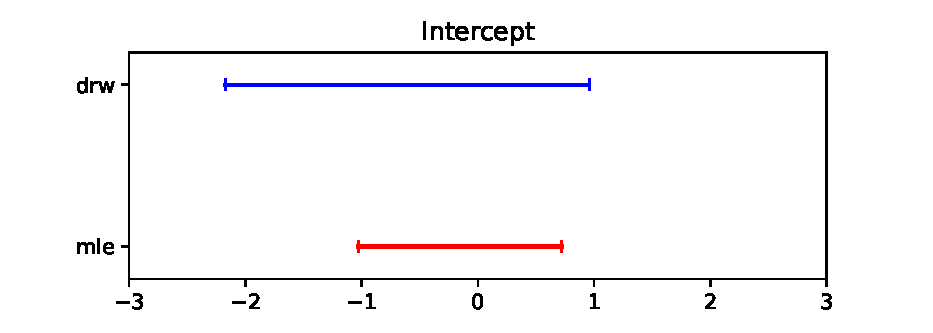
\includegraphics[width=\linewidth]{0.eps}
\end{minipage}
\begin{minipage}{0.48\linewidth}
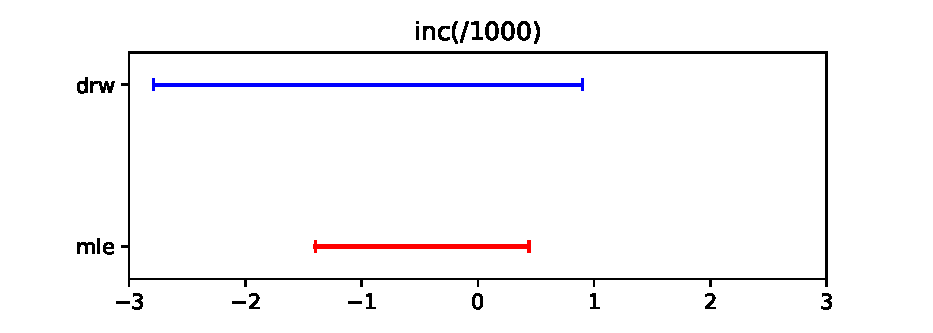
\includegraphics[width=\linewidth]{1.eps}
\end{minipage}
\begin{minipage}{0.48\linewidth}
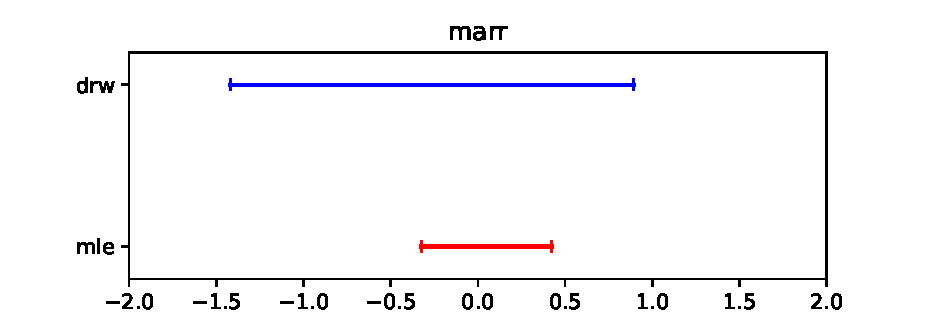
\includegraphics[width=\linewidth]{2.eps}
\end{minipage}
\begin{minipage}{0.48\linewidth}
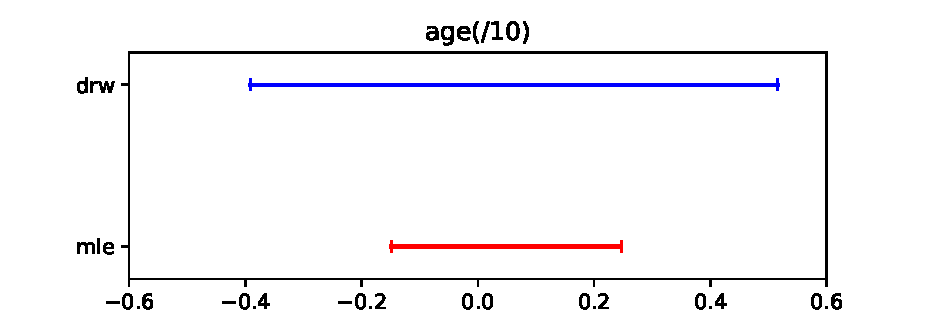
\includegraphics[width=\linewidth]{3.eps}
\end{minipage}
\begin{minipage}{0.48\linewidth}
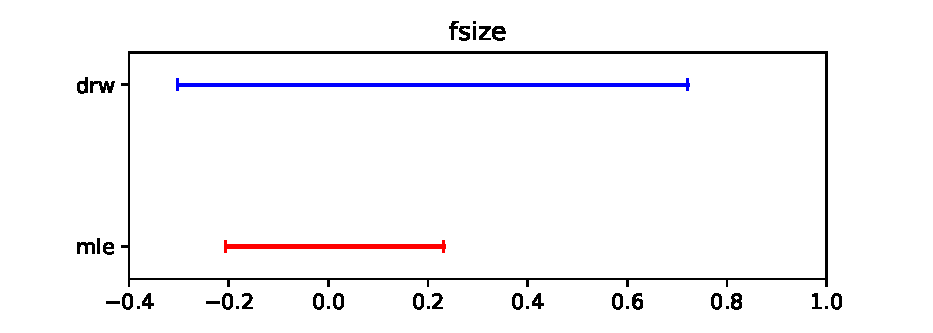
\includegraphics[width=\linewidth]{4.eps}
\end{minipage}
\begin{minipage}{0.48\linewidth}
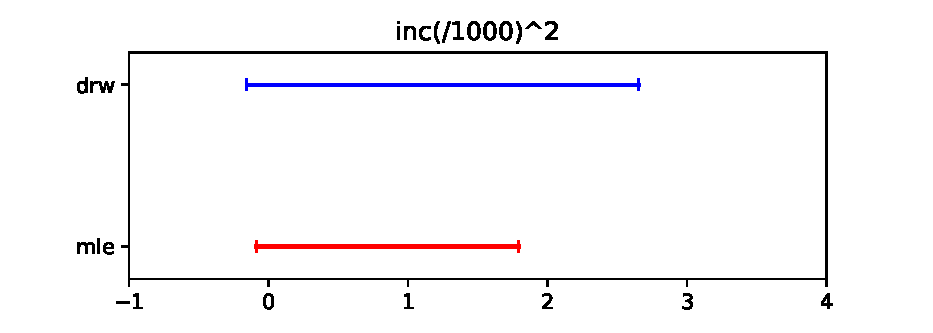
\includegraphics[width=\linewidth]{5.eps}
\end{minipage}
\caption{95\% Confidence intervals of estimates of coefficients in $\delta^{\mathrm{M}}$ using different methods (Repeated by us)}
\end{figure}

\begin{figure}
\centering
\begin{minipage}{0.48\linewidth}
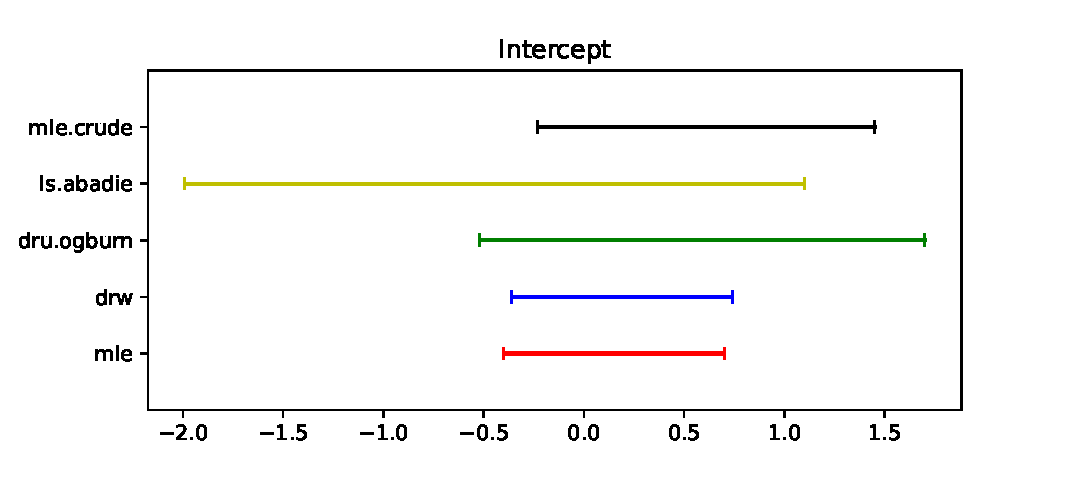
\includegraphics[width=\linewidth]{all0.eps}
\end{minipage}
\begin{minipage}{0.48\linewidth}
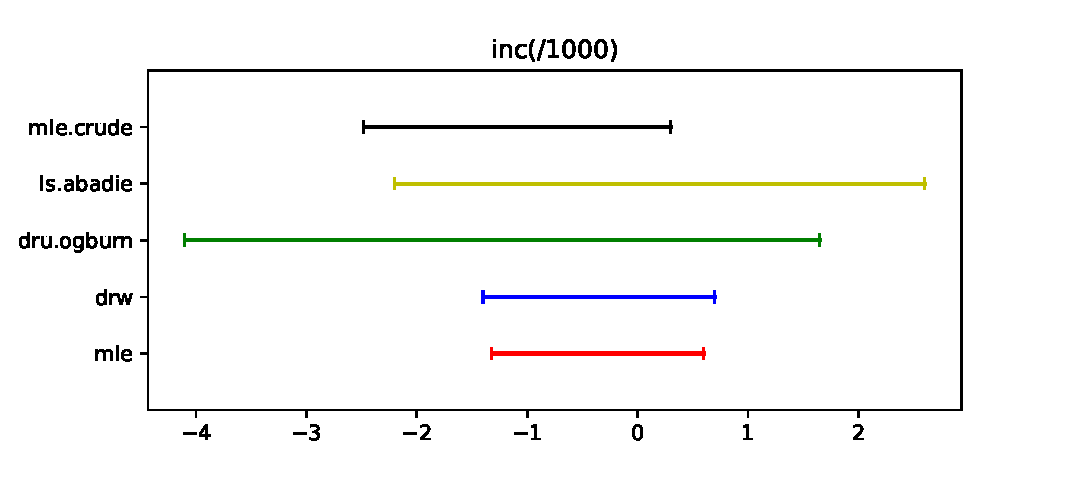
\includegraphics[width=\linewidth]{all1.eps}
\end{minipage}
\begin{minipage}{0.48\linewidth}
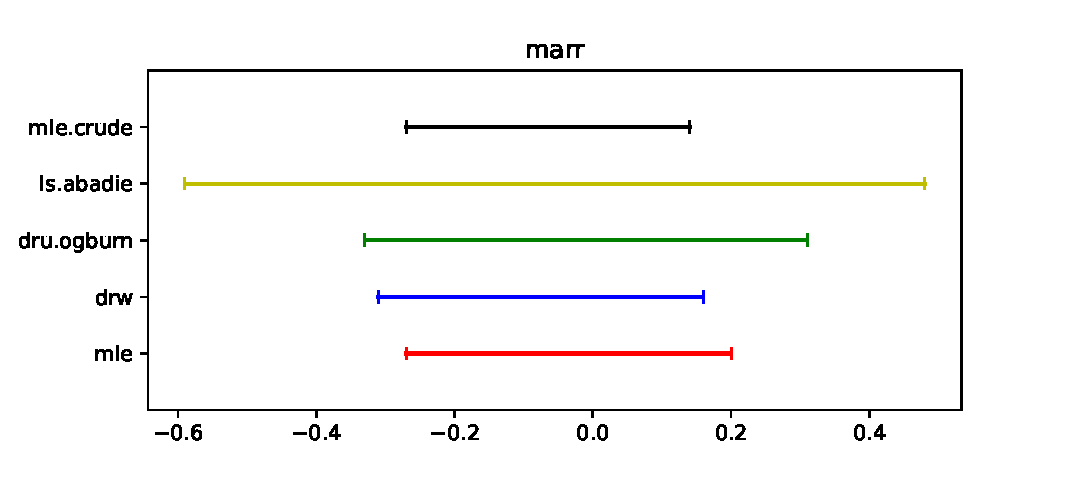
\includegraphics[width=\linewidth]{all2.eps}
\end{minipage}
\begin{minipage}{0.48\linewidth}
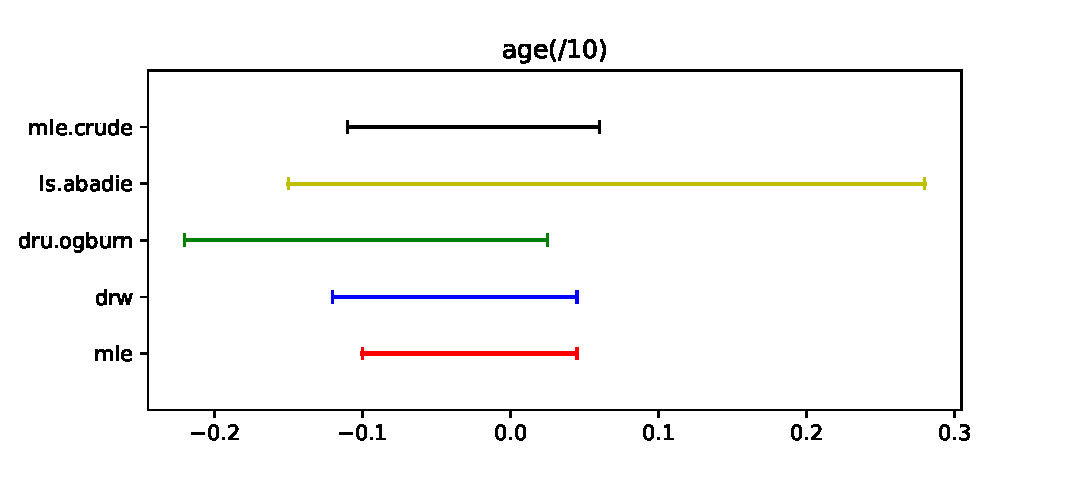
\includegraphics[width=\linewidth]{all3.eps}
\end{minipage}
\begin{minipage}{0.48\linewidth}
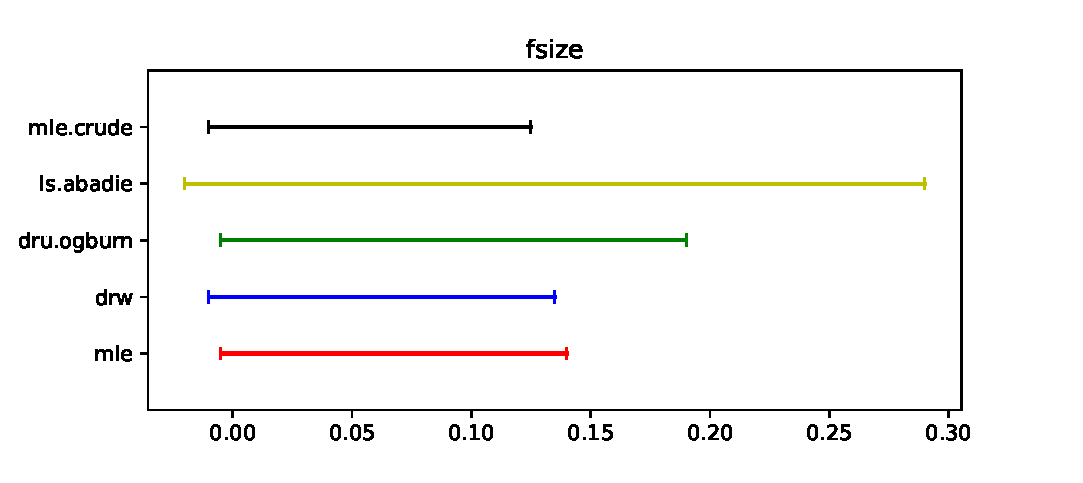
\includegraphics[width=\linewidth]{all4.eps}
\end{minipage}
\begin{minipage}{0.48\linewidth}
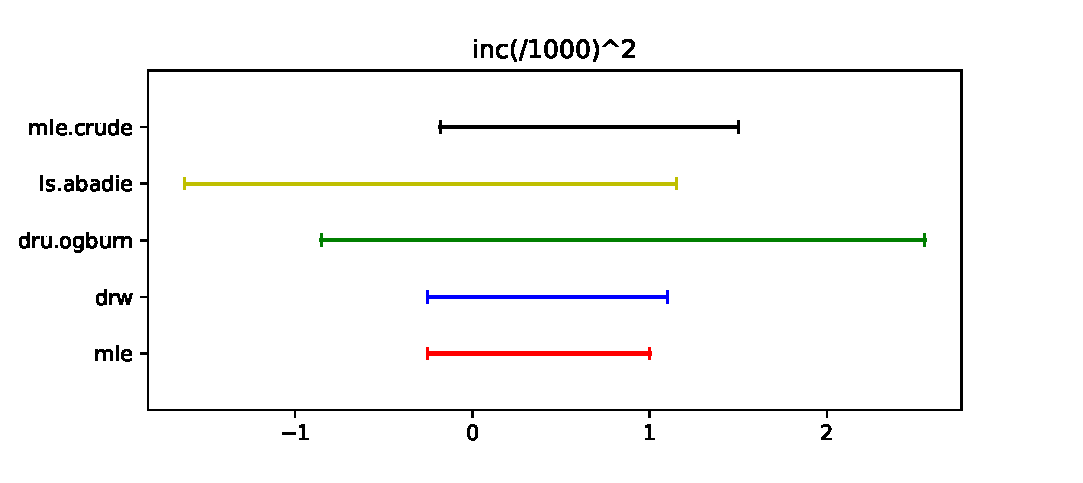
\includegraphics[width=\linewidth]{all5.eps}
\end{minipage}
\caption{95\% Confidence intervals of estimates of coefficients in $\delta^{\mathrm{M}}$ using different methods (Reported by ARTICLE)}
\end{figure}
% Table $2 .$ Bias $(\times 100)$ and standard error $(\times 100$, in parentheses $)$ of the estimated biases in the Monte Carlo study of various estimators in the selected scenarios; the true values of $\alpha$ c and $\alpha_{1}$ are 0 and $-1$, respectively, and the sample size is 1000
% $$
% \begin{aligned}
% \delta^{\mathrm{L}}(X) &=\tanh \left(\alpha^{\mathrm{T}} X\right), \quad \delta^{\mathrm{M}}(X)=\exp \left(\alpha^{\mathrm{T}} X\right) \\
% \phi_{i}(X) &=\operatorname{expit}\left(\beta_{i}^{\mathrm{T}} X\right)(i=1, \ldots, 4), \quad{ }_{\mathrm{OP}}{ }^{\mathrm{CO}}(X)=\exp \left(\eta^{\mathrm{T}} X\right) \\
% \operatorname{pr}(Z=1 \mid X) &=\operatorname{expit}\left(\gamma^{\mathrm{T}} X\right)
% \end{aligned}
% $$
% where the covariates $X$ include an intercept and a random variable generated from $\operatorname{Un}(-1,1)$, $\alpha=(0,-1)^{\mathrm{T}}, \beta_{i}=(-0.4,0.8)^{\mathrm{T}}(i=1, \ldots, 4), \eta=(-0.4,1)^{\mathrm{T}}$ and $\gamma=(0.1,-1)^{\mathrm{T}}$. Under this setting, the strength of the instrumental variable, defined as $\Delta^{D}=E\{E(D \mid Z=1, X)-E(D \mid Z=$ $0, X)\}$, is $0.406$. The sample size is 1000 .

% We also consider scenarios in which the nuisance models are misspecified. In these scenarios, the analyst is given covariates $X^{\dagger}$ that include an intercept and an irrelevant covariate generated from an independent Un $(-1,1)$, as well as covariates $X^{\prime}$ including
% $$
% (\underbrace{1, \ldots, 1}_{0.5 n}, \underbrace{0 \ldots, 0}_{0.5 n})^{\mathrm{T}}, \quad(\underbrace{0, \ldots, 0}_{0.1 n}, \underbrace{1, \ldots, 1}_{0.9 n})^{\mathrm{T}} .
% $$
% Instead of formulating a model conditioning on $X$, the analyst fits the model $\operatorname{pr}\left(Z=1 \mid X^{\dagger} ; \gamma\right)$ and/or $\phi_{i}\left(X^{\prime} ; \beta_{i}\right)(i=1, \ldots, 4)$ and $\mathrm{OP}^{\mathrm{CO}}\left(X^{\prime} ; \eta\right)$. The analyst still uses the correct functional form in these models. The target model $\theta(X ; \alpha)$ is always correctly specified. In the Supplementary Material we visualize the degree of model misspecification by plotting the data points generated under the true models and misspecified models from one randomly selected Monte Carlo run.
% We assess the performance of the following estimators.
% mle: the proposed maximum likelihood estimator;
% drw: the proposed doubly robust estimator with the optimal weighting function;
% dru: the proposed doubly robust estimator with the identity weighting function;
% reg.ogburn: the outcome regression estimator of Ogburn et al. $(2015, \S 3.1)$;
% drw.ogburn: the doubly robust estimator of Ogburn et al. (2015, $\S 3.3$ )
% with the optimal weighting function;

\section{Submission of papers to NeurIPS 2022}


Please read the instructions below carefully and follow them faithfully.


\subsection{Style}


Papers to be submitted to NeurIPS 2022 must be prepared according to the
instructions presented here. Papers may only be up to {\bf nine} pages long,
including figures. Additional pages \emph{containing only acknowledgments and
references} are allowed. Papers that exceed the page limit will not be
reviewed, or in any other way considered for presentation at the conference.


The margins in 2022 are the same as those in 2007, which allow for $\sim$$15\%$
more words in the paper compared to earlier years.


Authors are required to use the NeurIPS \LaTeX{} style files obtainable at the
NeurIPS website as indicated below. Please make sure you use the current files
and not previous versions. Tweaking the style files may be grounds for
rejection.


\subsection{Retrieval of style files}


The style files for NeurIPS and other conference information are available on
the World Wide Web at
\begin{center}
  \url{http://www.neurips.cc/}
\end{center}
The file \verb+neurips_2022.pdf+ contains these instructions and illustrates the
various formatting requirements your NeurIPS paper must satisfy.


The only supported style file for NeurIPS 2022 is \verb+neurips_2022.sty+,
rewritten for \LaTeXe{}.  \textbf{Previous style files for \LaTeX{} 2.09,
  Microsoft Word, and RTF are no longer supported!}


The \LaTeX{} style file contains three optional arguments: \verb+final+, which
creates a camera-ready copy, \verb+preprint+, which creates a preprint for
submission to, e.g., arXiv, and \verb+nonatbib+, which will not load the
\verb+natbib+ package for you in case of package clash.


\paragraph{Preprint option}
If you wish to post a preprint of your work online, e.g., on arXiv, using the
NeurIPS style, please use the \verb+preprint+ option. This will create a
nonanonymized version of your work with the text ``Preprint. Work in progress.''
in the footer. This version may be distributed as you see fit. Please \textbf{do
  not} use the \verb+final+ option, which should \textbf{only} be used for
papers accepted to NeurIPS.


At submission time, please omit the \verb+final+ and \verb+preprint+
options. This will anonymize your submission and add line numbers to aid
review. Please do \emph{not} refer to these line numbers in your paper as they
will be removed during generation of camera-ready copies.


The file \verb+neurips_2022.tex+ may be used as a ``shell'' for writing your
paper. All you have to do is replace the author, title, abstract, and text of
the paper with your own.


The formatting instructions contained in these style files are summarized in
Sections \ref{gen_inst}, \ref{headings}, and \ref{others} below.


\section{General formatting instructions}
\label{gen_inst}


The text must be confined within a rectangle 5.5~inches (33~picas) wide and
9~inches (54~picas) long. The left margin is 1.5~inch (9~picas).  Use 10~point
type with a vertical spacing (leading) of 11~points.  Times New Roman is the
preferred typeface throughout, and will be selected for you by default.
Paragraphs are separated by \nicefrac{1}{2}~line space (5.5 points), with no
indentation.


The paper title should be 17~point, initial caps/lower case, bold, centered
between two horizontal rules. The top rule should be 4~points thick and the
bottom rule should be 1~point thick. Allow \nicefrac{1}{4}~inch space above and
below the title to rules. All pages should start at 1~inch (6~picas) from the
top of the page.


For the final version, authors' names are set in boldface, and each name is
centered above the corresponding address. The lead author's name is to be listed
first (left-most), and the co-authors' names (if different address) are set to
follow. If there is only one co-author, list both author and co-author side by
side.


Please pay special attention to the instructions in Section \ref{others}
regarding figures, tables, acknowledgments, and references.


\section{Headings: first level}
\label{headings}


All headings should be lower case (except for first word and proper nouns),
flush left, and bold.


First-level headings should be in 12-point type.


\subsection{Headings: second level}


Second-level headings should be in 10-point type.


\subsubsection{Headings: third level}


Third-level headings should be in 10-point type.


\paragraph{Paragraphs}


There is also a \verb+\paragraph+ command available, which sets the heading in
bold, flush left, and inline with the text, with the heading followed by 1\,em
of space.


\section{Citations, figures, tables, references}
\label{others}


These instructions apply to everyone.


\subsection{Citations within the text}


The \verb+natbib+ package will be loaded for you by default.  Citations may be
author/year or numeric, as long as you maintain internal consistency.  As to the
format of the references themselves, any style is acceptable as long as it is
used consistently.


The documentation for \verb+natbib+ may be found at
\begin{center}
  \url{http://mirrors.ctan.org/macros/latex/contrib/natbib/natnotes.pdf}
\end{center}
Of note is the command \verb+\citet+, which produces citations appropriate for
use in inline text.  For example,
\begin{verbatim}
   \citet{hasselmo} investigated\dots
\end{verbatim}
produces
\begin{quote}
  Hasselmo, et al.\ (1995) investigated\dots
\end{quote}


If you wish to load the \verb+natbib+ package with options, you may add the
following before loading the \verb+neurips_2022+ package:
\begin{verbatim}
   \PassOptionsToPackage{options}{natbib}
\end{verbatim}


If \verb+natbib+ clashes with another package you load, you can add the optional
argument \verb+nonatbib+ when loading the style file:
\begin{verbatim}
   \usepackage[nonatbib]{neurips_2022}
\end{verbatim}


As submission is double blind, refer to your own published work in the third
person. That is, use ``In the previous work of Jones et al.\ [4],'' not ``In our
previous work [4].'' If you cite your other papers that are not widely available
(e.g., a journal paper under review), use anonymous author names in the
citation, e.g., an author of the form ``A.\ Anonymous.''


\subsection{Footnotes}


Footnotes should be used sparingly.  If you do require a footnote, indicate
footnotes with a number\footnote{Sample of the first footnote.} in the
text. Place the footnotes at the bottom of the page on which they appear.
Precede the footnote with a horizontal rule of 2~inches (12~picas).


Note that footnotes are properly typeset \emph{after} punctuation
marks.\footnote{As in this example.}


\subsection{Figures}


\begin{figure}
  \centering
  \fbox{\rule[-.5cm]{0cm}{4cm} \rule[-.5cm]{4cm}{0cm}}
  \caption{Sample figure caption.}
\end{figure}


All artwork must be neat, clean, and legible. Lines should be dark enough for
purposes of reproduction. The figure number and caption always appear after the
figure. Place one line space before the figure caption and one line space after
the figure. The figure caption should be lower case (except for first word and
proper nouns); figures are numbered consecutively.


You may use color figures.  However, it is best for the figure captions and the
paper body to be legible if the paper is printed in either black/white or in
color.


\subsection{Tables}


All tables must be centered, neat, clean and legible.  The table number and
title always appear before the table.  See Table~\ref{sample-table}.


Place one line space before the table title, one line space after the
table title, and one line space after the table. The table title must
be lower case (except for first word and proper nouns); tables are
numbered consecutively.


Note that publication-quality tables \emph{do not contain vertical rules.} We
strongly suggest the use of the \verb+booktabs+ package, which allows for
typesetting high-quality, professional tables:
\begin{center}
  \url{https://www.ctan.org/pkg/booktabs}
\end{center}
This package was used to typeset Table~\ref{sample-table}.


\begin{table}
  \caption{Sample table title}
  \label{sample-table}
  \centering
  \begin{tabular}{lll}
    \toprule
    \multicolumn{2}{c}{Part}                   \\
    \cmidrule(r){1-2}
    Name     & Description     & Size ($\mu$m) \\
    \midrule
    Dendrite & Input terminal  & $\sim$100     \\
    Axon     & Output terminal & $\sim$10      \\
    Soma     & Cell body       & up to $10^6$  \\
    \bottomrule
  \end{tabular}
\end{table}


\section{Final instructions}


Do not change any aspects of the formatting parameters in the style files.  In
particular, do not modify the width or length of the rectangle the text should
fit into, and do not change font sizes (except perhaps in the
\textbf{References} section; see below). Please note that pages should be
numbered.


\section{Preparing PDF files}


Please prepare submission files with paper size ``US Letter,'' and not, for
example, ``A4.''


Fonts were the main cause of problems in the past years. Your PDF file must only
contain Type 1 or Embedded TrueType fonts. Here are a few instructions to
achieve this.


\begin{itemize}


\item You should directly generate PDF files using \verb+pdflatex+.


\item You can check which fonts a PDF files uses.  In Acrobat Reader, select the
  menu Files$>$Document Properties$>$Fonts and select Show All Fonts. You can
  also use the program \verb+pdffonts+ which comes with \verb+xpdf+ and is
  available out-of-the-box on most Linux machines.


\item The IEEE has recommendations for generating PDF files whose fonts are also
  acceptable for NeurIPS. Please see
  \url{http://www.emfield.org/icuwb2010/downloads/IEEE-PDF-SpecV32.pdf}


\item \verb+xfig+ "patterned" shapes are implemented with bitmap fonts.  Use
  "solid" shapes instead.


\item The \verb+\bbold+ package almost always uses bitmap fonts.  You should use
  the equivalent AMS Fonts:
\begin{verbatim}
   \usepackage{amsfonts}
\end{verbatim}
followed by, e.g., \verb+\mathbb{R}+, \verb+\mathbb{N}+, or \verb+\mathbb{C}+
for $\mathbb{R}$, $\mathbb{N}$ or $\mathbb{C}$.  You can also use the following
workaround for reals, natural and complex:
\begin{verbatim}
   \newcommand{\RR}{I\!\!R} %real numbers
   \newcommand{\Nat}{I\!\!N} %natural numbers
   \newcommand{\CC}{I\!\!\!\!C} %complex numbers
\end{verbatim}
Note that \verb+amsfonts+ is automatically loaded by the \verb+amssymb+ package.


\end{itemize}


If your file contains type 3 fonts or non embedded TrueType fonts, we will ask
you to fix it.


\subsection{Margins in \LaTeX{}}


Most of the margin problems come from figures positioned by hand using
\verb+\special+ or other commands. We suggest using the command
\verb+\includegraphics+ from the \verb+graphicx+ package. Always specify the
figure width as a multiple of the line width as in the example below:
\begin{verbatim}
   \usepackage[pdftex]{graphicx} ...
   \includegraphics[width=0.8\linewidth]{myfile.pdf}
\end{verbatim}
See Section 4.4 in the graphics bundle documentation
(\url{http://mirrors.ctan.org/macros/latex/required/graphics/grfguide.pdf})


A number of width problems arise when \LaTeX{} cannot properly hyphenate a
line. Please give LaTeX hyphenation hints using the \verb+\-+ command when
necessary.


\begin{ack}
Use unnumbered first level headings for the acknowledgments. All acknowledgments
go at the end of the paper before the list of references. Moreover, you are required to declare
funding (financial activities supporting the submitted work) and competing interests (related financial activities outside the submitted work).
More information about this disclosure can be found at: \url{https://neurips.cc/Conferences/2022/PaperInformation/FundingDisclosure}.


Do {\bf not} include this section in the anonymized submission, only in the final paper. You can use the \texttt{ack} environment provided in the style file to autmoatically hide this section in the anonymized submission.
\end{ack}


\section*{References}

References follow the acknowledgments. Use unnumbered first-level heading for
the references. Any choice of citation style is acceptable as long as you are
consistent. It is permissible to reduce the font size to \verb+small+ (9 point)
when listing the references.
Note that the Reference section does not count towards the page limit.
\medskip

{
\small

% \begin{thebibliography}{99} 
% \bibitem{hello} [1] Wang, L., Zhang, Y., Richardson, T. S., \& Robins, J. M. (2021). Estimation of local treatment effects under the binary instrumental variable model. {\it Biometrika}, 108(4), 881-894.
% \end{thebibliography}
[1] Wang, L., Zhang, Y., Richardson, T. S., \& Robins, J. M. (2021). Estimation of local treatment effects under the binary instrumental variable model. {\it Biometrika}, 108(4), 881-894.

[2] Bower, J.M.\ \& Beeman, D.\ (1995) {\it The Book of GENESIS: Exploring
  Realistic Neural Models with the GEneral NEural SImulation System.}  New York:
TELOS/Springer--Verlag.


[3] Hasselmo, M.E., Schnell, E.\ \& Barkai, E.\ (1995) Dynamics of learning and
recall at excitatory recurrent synapses and cholinergic modulation in rat
hippocampal region CA3. {\it Journal of Neuroscience} {\bf 15}(7):5249-5262.
}


%%%%%%%%%%%%%%%%%%%%%%%%%%%%%%%%%%%%%%%%%%%%%%%%%%%%%%%%%%%%
\section*{Checklist}


%%% BEGIN INSTRUCTIONS %%%
The checklist follows the references.  Please
read the checklist guidelines carefully for information on how to answer these
questions.  For each question, change the default \answerTODO{} to \answerYes{},
\answerNo{}, or \answerNA{}.  You are strongly encouraged to include a {\bf
justification to your answer}, either by referencing the appropriate section of
your paper or providing a brief inline description.  For example:
\begin{itemize}
  \item Did you include the license to the code and datasets? \answerYes{See Section~\ref{gen_inst}.}
  \item Did you include the license to the code and datasets? \answerNo{The code and the data are proprietary.}
  \item Did you include the license to the code and datasets? \answerNA{}
\end{itemize}
Please do not modify the questions and only use the provided macros for your
answers.  Note that the Checklist section does not count towards the page
limit.  In your paper, please delete this instructions block and only keep the
Checklist section heading above along with the questions/answers below.
%%% END INSTRUCTIONS %%%


\begin{enumerate}


\item For all authors...
\begin{enumerate}
  \item Do the main claims made in the abstract and introduction accurately reflect the paper's contributions and scope?
    \answerTODO{}
  \item Did you describe the limitations of your work?
    \answerTODO{}
  \item Did you discuss any potential negative societal impacts of your work?
    \answerTODO{}
  \item Have you read the ethics review guidelines and ensured that your paper conforms to them?
    \answerTODO{}
\end{enumerate}


\item If you are including theoretical results...
\begin{enumerate}
  \item Did you state the full set of assumptions of all theoretical results?
    \answerTODO{}
        \item Did you include complete proofs of all theoretical results?
    \answerTODO{}
\end{enumerate}


\item If you ran experiments...
\begin{enumerate}
  \item Did you include the code, data, and instructions needed to reproduce the main experimental results (either in the supplemental material or as a URL)?
    \answerTODO{}
  \item Did you specify all the training details (e.g., data splits, hyperparameters, how they were chosen)?
    \answerTODO{}
        \item Did you report error bars (e.g., with respect to the random seed after running experiments multiple times)?
    \answerTODO{}
        \item Did you include the total amount of compute and the type of resources used (e.g., type of GPUs, internal cluster, or cloud provider)?
    \answerTODO{}
\end{enumerate}


\item If you are using existing assets (e.g., code, data, models) or curating/releasing new assets...
\begin{enumerate}
  \item If your work uses existing assets, did you cite the creators?
    \answerTODO{}
  \item Did you mention the license of the assets?
    \answerTODO{}
  \item Did you include any new assets either in the supplemental material or as a URL?
    \answerTODO{}
  \item Did you discuss whether and how consent was obtained from people whose data you're using/curating?
    \answerTODO{}
  \item Did you discuss whether the data you are using/curating contains personally identifiable information or offensive content?
    \answerTODO{}
\end{enumerate}


\item If you used crowdsourcing or conducted research with human subjects...
\begin{enumerate}
  \item Did you include the full text of instructions given to participants and screenshots, if applicable?
    \answerTODO{}
  \item Did you describe any potential participant risks, with links to Institutional Review Board (IRB) approvals, if applicable?
    \answerTODO{}
  \item Did you include the estimated hourly wage paid to participants and the total amount spent on participant compensation?
    \answerTODO{}
\end{enumerate}


\end{enumerate}


%%%%%%%%%%%%%%%%%%%%%%%%%%%%%%%%%%%%%%%%%%%%%%%%%%%%%%%%%%%%


\appendix


\section{Appendix}


Optionally include extra information (complete proofs, additional experiments and plots) in the appendix.
This section will often be part of the supplemental material.


\end{document}
